\documentclass[12pt]{article}
\usepackage[utf8]{inputenc}
\usepackage{tabularx}
\usepackage{booktabs}
\usepackage{graphicx}
\usepackage{siunitx}
\usepackage{titlesec}
\usepackage[shortlabels]{enumitem}
\usepackage[round]{natbib}
\usepackage{array}

%% Comments

\usepackage{color}

\newif\ifcomments\commentstrue %displays comments
%\newif\ifcomments\commentsfalse %so that comments do not display

\ifcomments
\newcommand{\authornote}[3]{\textcolor{#1}{[#3 ---#2]}}
\newcommand{\todo}[1]{\textcolor{red}{[TODO: #1]}}
\else
\newcommand{\authornote}[3]{}
\newcommand{\todo}[1]{}
\fi

\newcommand{\wss}[1]{\authornote{blue}{SS}{#1}} 
\newcommand{\plt}[1]{\authornote{magenta}{TPLT}{#1}} %For explanation of the template
\newcommand{\an}[1]{\authornote{cyan}{Author}{#1}}

%% Common Parts

\newcommand{\progname}{Chess Connect} % PUT YOUR PROGRAM NAME HERE
\newcommand{\authname}{Team \#4,
\\ Alexander Van Kralingen
\\ Arshdeep Aujla
\\ Jonathan Cels
\\ Joshua Chapman
\\ Rupinder Nagra} % AUTHOR NAMES without MacIDs 

\usepackage{hyperref}
    \hypersetup{colorlinks=true, linkcolor=blue, citecolor=blue, filecolor=blue,
                urlcolor=blue, unicode=false}
    \urlstyle{same}
                                


\setcounter{secnumdepth}{4}

\titleformat{\paragraph}
{\normalfont\normalsize\bfseries}{\theparagraph}{1em}{}
\titlespacing*{\paragraph}
{0pt}{3.25ex plus 1ex minus .2ex}{1.5ex plus .2ex}

\begin{document}

\title{Software Requirements Specification for Chess Connect: Online tools combined with on-board vision to improve and share your game} 
\author{\authname}
\date{October 4th, 2022}
	
\maketitle

~\newpage

\tableofcontents

~\newpage

\addcontentsline{toc}{section}{Table of Revisions}
\section*{Table of Revisions}
\begin{table}[hp]
\caption{Revision History} \label{TblRevisionHistory}
\begin{tabularx}{\textwidth}{llX}
\toprule
\textbf{Date} & \textbf{Developer(s)} & \textbf{Change}\\
\midrule
2022-10-04 & Jonathan Cels & Template creation and document formatting\\ 
2022-10-04 & Jonathan Cels & Non-functional requirements\\
2022-10-05 & Alexander Van Kralingen & Added Context Diagram\\
date & name & change\\
\bottomrule
\end{tabularx}
\end{table}

~\newpage

\section{Units, Terms, Acronyms, and Abbreviations}

\subsection{Table of Units}
Throughout this document SI (Syst\`{e}me International d'Unit\'{e}s) is employed
as the unit system.  In addition to the basic units, several derived units are
used as described below.  For each unit, the symbol is given followed by a
description of the unit and the SI name.

\begin{table}[ht]
  \noindent \begin{tabular}{l l l} 
    \toprule		
    \textbf{symbol} & \textbf{unit} & \textbf{SI}\\
    \midrule 
    \si{\volt} & electric potential & volt\\
    \si{\ampere} & current	& ampere\\
    \si{\ohm} & resistance	& ohm\\
    \si{\second} & time & second\\
    \si{\celsius} & temperature & centigrade\\
    \si{\joule} & energy & joule\\
    \si{\watt} & power & watt (W = \si{\joule\per\second})\\
    \bottomrule
  \end{tabular}
\end{table}

\newpage

\subsection{Abbreviations and Acronyms}
\begin{tabular}{l l} 
  \toprule		
  \textbf{symbol} & \textbf{description}\\
  \midrule 
  A & Assumption\\
  CSA & Canadian Standards Association\\
  DD & Data Definition\\
  FIDE & International Chess Federation or Fédération Internationale des Échecs\\
  GD & General Definition\\
  GS & Goal Statement\\
  IM & Instance Model\\
  LC & Likely Change\\
  LCD & Liquid Crystal Display\\
  LED & Light-Emmitting Diode\\
  MCU & Micro Controller Unit\\
  PS & Physical System Description\\
  R & Requirement\\
  SRS & Software Requirements Specification\\
  T & Theoretical Model\\
  VnV & Verification and Validation\\
  WCAG & Web Content Accessibility Guidelines\\
  \bottomrule
\end{tabular}\\

\subsection{Mathematical Notation}

\subsection{Terminology and  Definitions}

\section{Introduction}
\subsection{Document Purpose}
\subsection{Characteristics of Intended Reader}
\subsection{Characteristics of Intended User}
\subsection{Stakeholders}

\section{Problem Description}

\section{Assumptions}

\section{Constraints}

\section{Scope}

\section{Project Overview}
\subsection{System Context Diagram}

The context of the system invloves two integrated but separate system components, as well as two distinct end users.

\begin{figure}[h!]
  \begin{center}
    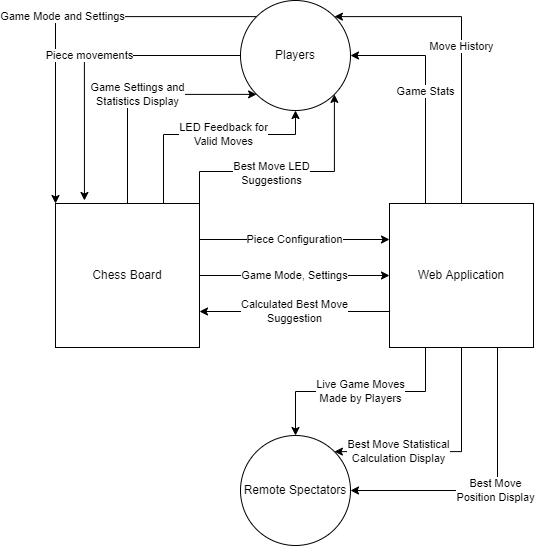
\includegraphics[scale=0.65]{chess-connect-system-context.png}
    \caption{System Context}
    \label{Fig_SystemContext} 
  \end{center}
\end{figure}

\subsection{Normal Operation}
\subsubsection{Description}
\subsubsection{Use Cases/Scenarios}

\subsection{Behaviour Overview}
\subsection{Undesired Scenario Handling}

\section{System Level Variables}
\subsection{Constants}
\subsection{Monitored Variables}
\subsection{Controlled Variables}

~\newpage

\section{Requirements}
\subsection{Functional Requirements}
\subsection{Nonfunctional Requirements}

\newcounter{vnvSectionNfr}
\setcounter{vnvSectionNfr}{1}

\newcounter{nfrNum}
\setcounter{nfrNum}{1}

\subsubsection{Look and Feel Requirements}
\label{NFR_LF}
\paragraph{Appearance Requirements}
\begin{enumerate}[{LF}1., leftmargin=2\parindent]
    \item The product shall use white, black, grey, and brown as its primary colours.
    \item The product shall use green, red, and blue as its secondary colours.
\end{enumerate}

\paragraph{Style Requirements}
\begin{enumerate}[{LF}1., leftmargin=2\parindent, resume]
    \item The product shall look and feel similar enough to traditional chess boards and chess pieces that the target audience will 
    recognize the product as a chess set when encountering it for the first time. The level and speed of audience recognition achieved 
    by the design shall be described following the procedure given in Section 5.2.\thevnvSectionNfr\stepcounter{vnvSectionNfr}~of the VnV 
    (Verification and Validation) Plan.
\end{enumerate}



\subsubsection{Usability and Humanity Requirements}
\label{NFR_UH}
\paragraph{Ease of Use Requirements}
\begin{enumerate}[{UH}1., leftmargin=2\parindent]
    \item The system shall require the user to place chess pieces fully on their intended squares.
    \item Physical hardware components of the system will not impede the user during play.
\end{enumerate}

\paragraph{Personalization and Internationalization Requirements}
\begin{enumerate}[{UH}1., leftmargin=2\parindent, resume]
    \item The system will only display information in English.
    \item The system will only use the Arabic numerals.
\end{enumerate}

\paragraph{Learning Requirements}
\begin{enumerate}[{UH}1., leftmargin=2\parindent, resume]
    \item The product shall be able to be used by members of the public over with no previous training. Details on the learnability 
    of the system shall be described following the procedure given in Section 5.2.\thevnvSectionNfr\stepcounter{vnvSectionNfr}
    of the VnV Plan.
\end{enumerate}

\paragraph{Understandability and Politeness Requirements}
\begin{enumerate}[{UH}1., leftmargin=2\parindent, resume]
    \item All symbols and words shall be similar to historically used Chess symbols. \cite{ChessHistory2003}
\end{enumerate}

\paragraph{Accessibility Requirements}
\begin{enumerate}[{UH}1., leftmargin=2\parindent, resume]
    \item The system shall follow guidelines for correct size and colour contrast ratio for text to the background as stated in the \cite{WCAG2018}.
\end{enumerate}



\subsubsection{Performance Requirements}
\label{NFR_PR}
\paragraph{Speed and Latency Requirements}
\begin{enumerate}[{PR}1., leftmargin=2\parindent]
    \item The average time between a user placing down a piece and the visual model response shall be small.
    \item The maximum time between a user placing down a piece and the visual model response shall be small.
    \item The average time between a user picking up a piece and the visual board indicator response shall be small.
    \item The maximum time between a user picking up a piece and the visual board indicator response shall be small. 
    The degree of speed for PR1 through PR4 shall be described following the procedure given in Section 5.2.\thevnvSectionNfr\stepcounter{vnvSectionNfr}
    of the VnV Plan.
\end{enumerate}

%Modified from Safety-Critical Requirements to better cover the SRS rubric
\paragraph{Health and Safety-Critical Requirements}
\begin{enumerate}[{PR}1., leftmargin=2\parindent, resume]
    \item The system shall be properly grounded according to the Canadian Electrical Code. \cite{CanadianElectricalCode2021}
    \item The maximum power on any single wire shall be within the safety limits described in the Canadian Electrical Code.
\end{enumerate}

\paragraph{Precision or Accuracy Requirements}
\begin{enumerate}[{PR}1., leftmargin=2\parindent, resume]
    \item The software application game state will model the game state on the \progname{} hardware with a high degree of accuracy. 
    The level of accuracy shall be described following the procedure given in Section 5.2.\thevnvSectionNfr\stepcounter{vnvSectionNfr}
    of the VnV Plan.
        
\end{enumerate}

\paragraph{Reliability and Availability Requirements}
\begin{enumerate}[{PR}1., leftmargin=2\parindent, resume]
    \item The product shall be available with a high degree of uptime. The level of availability shall be described following the procedure 
    given in Section 5.2.\thevnvSectionNfr\stepcounter{vnvSectionNfr} of the VnV Plan.
\end{enumerate}

\paragraph{Robustness or Fault-Tolerance Requirements}
\begin{enumerate}[{PR}1., leftmargin=2\parindent, resume]
    \item The software application shall maintain the game state if the connection between the software and hardware systems is interrupted.
\end{enumerate}

\paragraph{Capacity Requirements}
\begin{enumerate}[{PR}1., leftmargin=2\parindent, resume]
    \item The software shall require computer memory to function effectively. The level of memory capacity required shall be described following
    the procedure given in Section 5.2.\thevnvSectionNfr\stepcounter{vnvSectionNfr} of the VnV Plan.
\end{enumerate}

\paragraph{Scalability or Extensibility Requirements}
\begin{enumerate}[{PR}1., leftmargin=2\parindent, resume]
    \item The product must support the addition of new features and components.
\end{enumerate}

\paragraph{Longevity Requirements}
\begin{enumerate}[{PR}1., leftmargin=2\parindent, resume]
    \item The product must be supported while the application remains deployed.
    \item The product will depend on the continued support of packages and libraries.
\end{enumerate}



\subsubsection{Operational and Environmental Requirements}
\label{NFR_OE}
\paragraph{Expected Physical Environment}
\begin{enumerate}[{OE}1., leftmargin=2\parindent]
    \item The hardware and software systems shall be close enough to each other to facilitate communication. The degree of proximity required 
    shall be described following the procedure given in Section 5.2.\thevnvSectionNfr\stepcounter{vnvSectionNfr} of the VnV Plan.
    \item The area shall be clear of potentially dangerous or harmful environmental factors.
\end{enumerate}

\paragraph{Requirements for Interfacing with Adjacent Systems}
\begin{enumerate}[{OE}1., leftmargin=2\parindent, resume]
    \item The system shall interface with an external server to make requests to a chess engine.
\end{enumerate}

\paragraph{Productization Requirements}
\begin{enumerate}[{OE}1., leftmargin=2\parindent, resume]
    \item The product shall be deployed to a public website where users may access it.
\end{enumerate}

\paragraph{Release Requirements}
\begin{enumerate}[{OE}1., leftmargin=2\parindent, resume]
    \item The product will be tested for bugs and issues. These issues will be fixed and the application will be redeployed accordingly.
\end{enumerate}



\subsubsection{Maintainability and Support Requirements}
\label{NFR_MS}
\paragraph{Maintenance Requirements}
\begin{enumerate}[{MS}1., leftmargin=2\parindent]
    \item The product shall be maintained actively by the developers until the \progname{} team graduates.
\end{enumerate}

\paragraph{Supportability Requirements}
N/A

\paragraph{Adaptability Requirements}
\begin{enumerate}[{MS}1., leftmargin=2\parindent, resume]
    \item The software application will be able to be hosted on Apple, Windows, and Linux devices.
    \item The product shall be accessible from any web browser.
\end{enumerate}



\subsubsection{Security Requirements}
\label{NFR_SR}
\paragraph{Access Requirements}
\begin{enumerate}[{SR}1., leftmargin=2\parindent]
    \item Only the \progname{} team are able to modify the software system.
\end{enumerate}

\paragraph{Integrity Requirements}
\begin{enumerate}[{SR}1., leftmargin=2\parindent, resume]
    \item The product will not store game data after a game has concluded.
\end{enumerate}

\paragraph{Privacy Requirements}
\begin{enumerate}[{SR}1., leftmargin=2\parindent, resume]
    \item The product will not store or collect user data.
\end{enumerate}

\paragraph{Audit Requirements}
\begin{enumerate}[{SR}1., leftmargin=2\parindent, resume]
    \item Requirements shall be easy to follow and verify against both the system and the VnV plan in order to facilitate regular inspections.
\end{enumerate}

\paragraph{Immunity Requirements}
N/A



\subsubsection{Political and Cultural Requirements}
\label{NFR_PC}
\paragraph{Cultural Requirements}
\begin{enumerate}[{PC}1., leftmargin=2\parindent]
    \item The product will not use and terms or symbols that are deemed offensive to any culture.
\end{enumerate}

\paragraph{Political Requirements}
N/A



\subsubsection{Legal Requirements}
\label{NFR_Legal}
\paragraph{Compliance Requirements}
\begin{enumerate}[{LR}1., leftmargin=2\parindent]
    \item The system shall comply with the Canadian Electrical Code \cite{CanadianElectricalCode2021}.
\end{enumerate}

\paragraph{Standards Requirements}
\begin{enumerate}[{LR}1., leftmargin=2\parindent, resume]
    \item The product shall follow \cite{WCAG2018}.
\end{enumerate}


\section{Likely Changes}
\section{Unlikely Changes}

\section{Traceability Matrix}

\appendix
\section{Values of Auxiliary Constants}

\newpage

\appendix
\section{Reflection}
\subsection{Skills for Success}
\subsection{Knowledge and Learning Approaches}

\newpage

\bibliographystyle {plainnat}
\bibliography {../../refs/References}
\end{document}